\chapter{Implementação}

Com a contribuição deste trabalho, deve ser possível que um usuário do Noosfero
consiga encontrar e seguir a atividade de usuários de alguma instância do Diaspora.
Os usuários remotos descobertos devem possuir um perfil limitado no Diaspora, para
que as publicações na rede de origem sejam replicadas no Noosfero.

A implementação destas funcionalidades deve cobrir os pontos a seguir.

\begin{itemize}
  \item{Descoberta de usuários em um \textit{pod} do Diaspora.}
  \item{Resposta às consultas das informações do servidor Noosfero e da identidade
        ou informações do perfil de usuários locais.}
  \item{Envio de mensagens Salmon públicas e privadas para transportar as entidades
        que representam a interação social ou publicações.}
  \item{Recebimento de mensagens públicas que transportam entidades que representam
        novas publicações, criando publicações locais respectivas.}
\end{itemize}

A documentação da biblioteca utilizada para a implementação do protocolo não cobre
todos os aspectos da especificação, portanto foi necessário instanciar dois
\textit{pods} locais do Diaspora para analisar a comunicação. A comunicação do
Diaspora depende que cada um dos \textit{pods} responda a HTTPS e seja capaz de
resolver os nomes dos demais servidores.

Para os testes desse trabalho foram utilizadas duas máquinas virtuais com Debian 8
em rede privada, com os nomes registrados no arquivo de \textit{hosts} para a
resolução local. Em cada uma das máquinas, o Diaspora foi servido por um servidor
NGINX com SSL configurado com um certificado auto-assinado. Para que a comunicação
não fosse prejudicada pela verificação dos certificados, eles foram manualmente
adicionados aos certificados reconhecidos em cada uma das máquinas.

\section{AUTENTICAÇÃO COM O DIASPORA}

A federação através do Diaspora foi planejada com base na implementação já existente
no Noosfero, que conta com um mecanismo de autenticação entre as redes. Por esse
motivo inicialmente se julgou necessário permitir a autenticação de usuários com
credenciais de redes Diaspora.

O Diaspora não disponibiliza nenhum \textit{endpoint} de \textit{login} em sua API,
mas implementa o papel de fornecedor de identidades OpenID Connect\footnote{O OpenID
Connect é um padrão de autenticação construído sobre a segunda versão do OAuth.
\url{http://openid.net/specs/openid-connect-core-1_0.html}}. Portanto, a fim de
utilizar as credenciais do Diaspora, é necessário que o Noosfero possa desempenhar o
papel de cliente OpenID.

Mesmo que o Noosfero também forneça identidades OpenID, ainda não seria possível
usar credenciais locais para a autenticação em \textit{pods} Diaspora, que utiliza
apenas estratégias de autenticação local. Isso reforçou a decisão de implementar
apenas a função de cliente OpenID por enquanto.

Ainda que o \textit{plugi-in} tenha sido implementado como parte deste trabalho, o
restante da federação não depende deste mecanismo de autenticação, já que os
usuários só interagem com o servidor remoto através de sua rede de origem.

\subsection{Desenvolvimento do plugin OpenID Client}

Apesar do Noosfero já oferecer suporte à autorização com OAuth 1.0 através de um
\textit{plugin}, foi necessário implementar o suporte ao OpenID. A decisão foi criar
um novo \textit{plugin} que transforme o Noosfero em um cliente OpenID.

A \textit{gem} openid\char`_connect foi utilizada na implementação do consumidor. A
biblioteca já oferece as diretrizes de descoberta, registro de clientes e
autenticação, todas interações que envolvem requisições HTTP ao servidor fornecedor.
Um perfil externo também é criado no Noosfero para armazenar algumas informações do
perfil remoto, como \textit{link} para o seu perfil, ou sua imagem do avatar.

Os passos realizados pelo \textit{plugin} na autenticação de um usuários são:

\begin{enumerate}
  \item{O usuário digita o endereço do fornecedor OpenID de sua escolha;}
  \item{O Noosfero tenta descobrir informações a respeito do provedor, solicitando
        informações do emissor de identidades;}
  \item{Caso a resposta do provedor seja válida, o Noosfero solicita o registro como
        um novo cliente, solicitando acesso a informações necessárias para a criação
        de um perfil externo;}
  \item{A requisição é redirecionada ao fornecedor OpenID, onde o usuário deve se
        autenticar, e revisar a solicitação enviada pelo Noosfero;}
  \item{Se o usuário se autenticar no seu provedor e aprovar as informações
        solicitadas, a resposta do servidor será usada na criação de um perfil
        externo, e o usuário será autenticado no Noosfero}
\end{enumerate}



\section{DESCOBERTA DE USUÁRIOS}

A especificação do Diaspora propõe a descoberta de usuários através do WebFinger
para a consulta de identidades, e do hCard para o compartilhamento das informações
do perfil. O protocolo ainda segue a implementação do WebFinger que responde em
formato XML, considerada legada.

\begin{figure}[h]
	\centering
		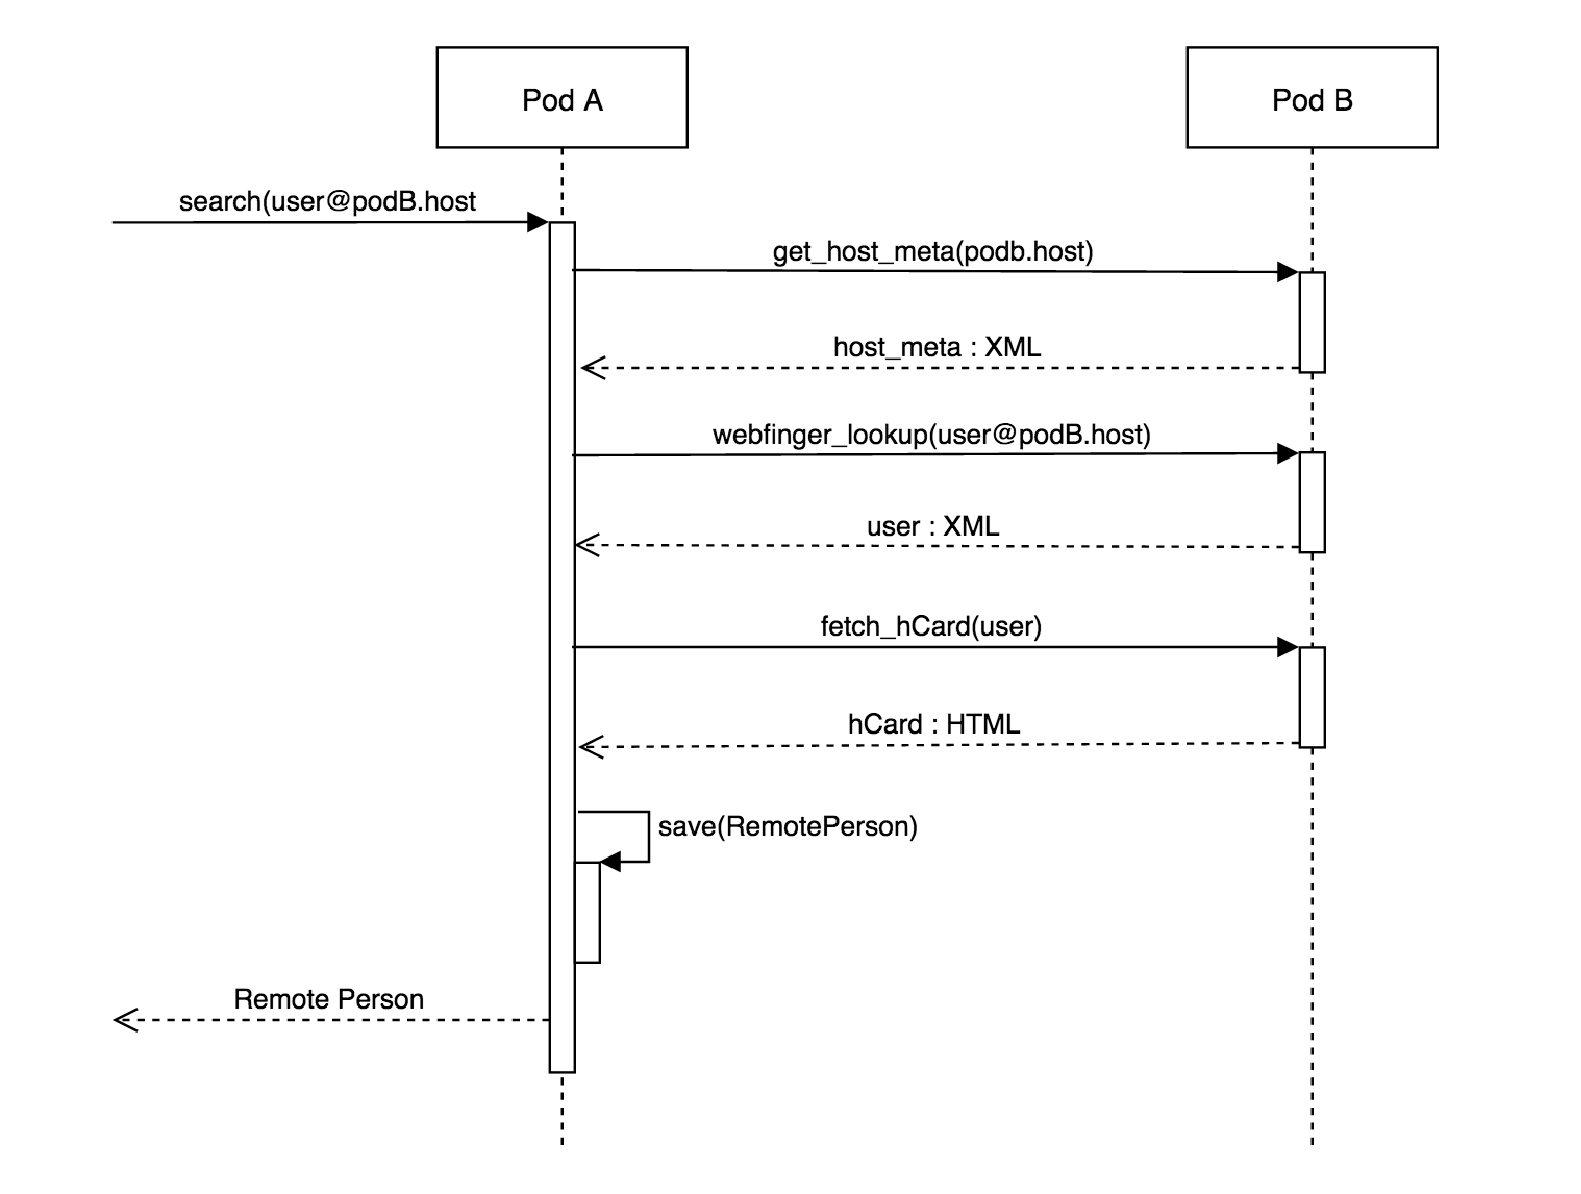
\includegraphics[keepaspectratio=true,scale=0.6]{figuras/seq_descoberta.eps}
	\caption{Diagrama de sequência do processo de descoberta de usuários}
	\label{fig:seq_descoberta}
\end{figure}

Como pode ser visto no diagrama da Figura \ref{fig:seq_descoberta}, o servidor
remoto é descoberto a partir de um identificador no formato \textit{nome do
usuário@servidor diaspora}. O \textit{endpoint} de descoberta de usuários deve ser
identificado através dos metadados do servidor remoto, também obtido através do
WebFinger, o qual será utilizado na consulta de identidade. A resposta às duas
requisições é formatada em XML. Após a descoberta de identidade, o servidor remoto é
novamente consultado pelo hCard do usuário, por sua vez em formato HTML, contendo as
informações do perfil público.

No Noosfero, a descoberta de usuários remotos foi implementada a partir da busca de
pessoas. Se a \textit{string} de busca conter o símbolo "@", a \textit{string} é
quebrada no formato \textit{nome@host}, e o processo descrito anteriormente é
executado para os atributos extraídos. Visto que trata-se de uma busca e os
resultados são imediatamente renderizados pelo servidor, por enquanto toda a
operação é realizada em \textit{foreground}.

Já que a implementação de descoberta é baseada no padrão WebFinger, apesar de seguir
o protocolo do Diaspora, é possível encontrar usuários em qualquer aplicação que o
implemente neste formato. Os \textit{endpoints} que respondem às requisições do
WebFinger e hCard foram implementadas como parte deste trabalho, e pode substituir
aos mecanismos atualmente implementados para a federação de redes Noosfero.

% TODO: no capítulo anterior falar por que motivo seria bom substituir
% - Separação do WebFinger só para descoberta -> hCard para compartilhar perfil


\section{TROCA DE MENSAGENS}

A primeira mudança introduzida no Noosfero foi a criação de páginas de perfil para
usuários externos, para conter as publicações resgatadas da rede de origem, e as
opções de interação. Anteriormente, referências a usuários remotos redirecionavam a
sua rede de origem. A criação de páginas locais exigiu alterações no mecanismo de
carregamento dos perfis no Noosfero. 

Para seguir um externo, é necessário enviar uma mensagem Salmon privada para o seu
\textit{endpoint} de recebimento. Ao receber esta mensagem, o Diaspora cria um
perfil remoto para o usuário do Noosfero que solicita a ação --- o que envolve a
obtenção de identidade e informações públicas na rede de origem, e registra as
informações a respeito do servidor. A Figura \ref{fig:seq_contato} descreve o
processo, que ocorre de maneira similar à executada durante a descoberta de
usuários.

\begin{figure}[h]
	\centering
		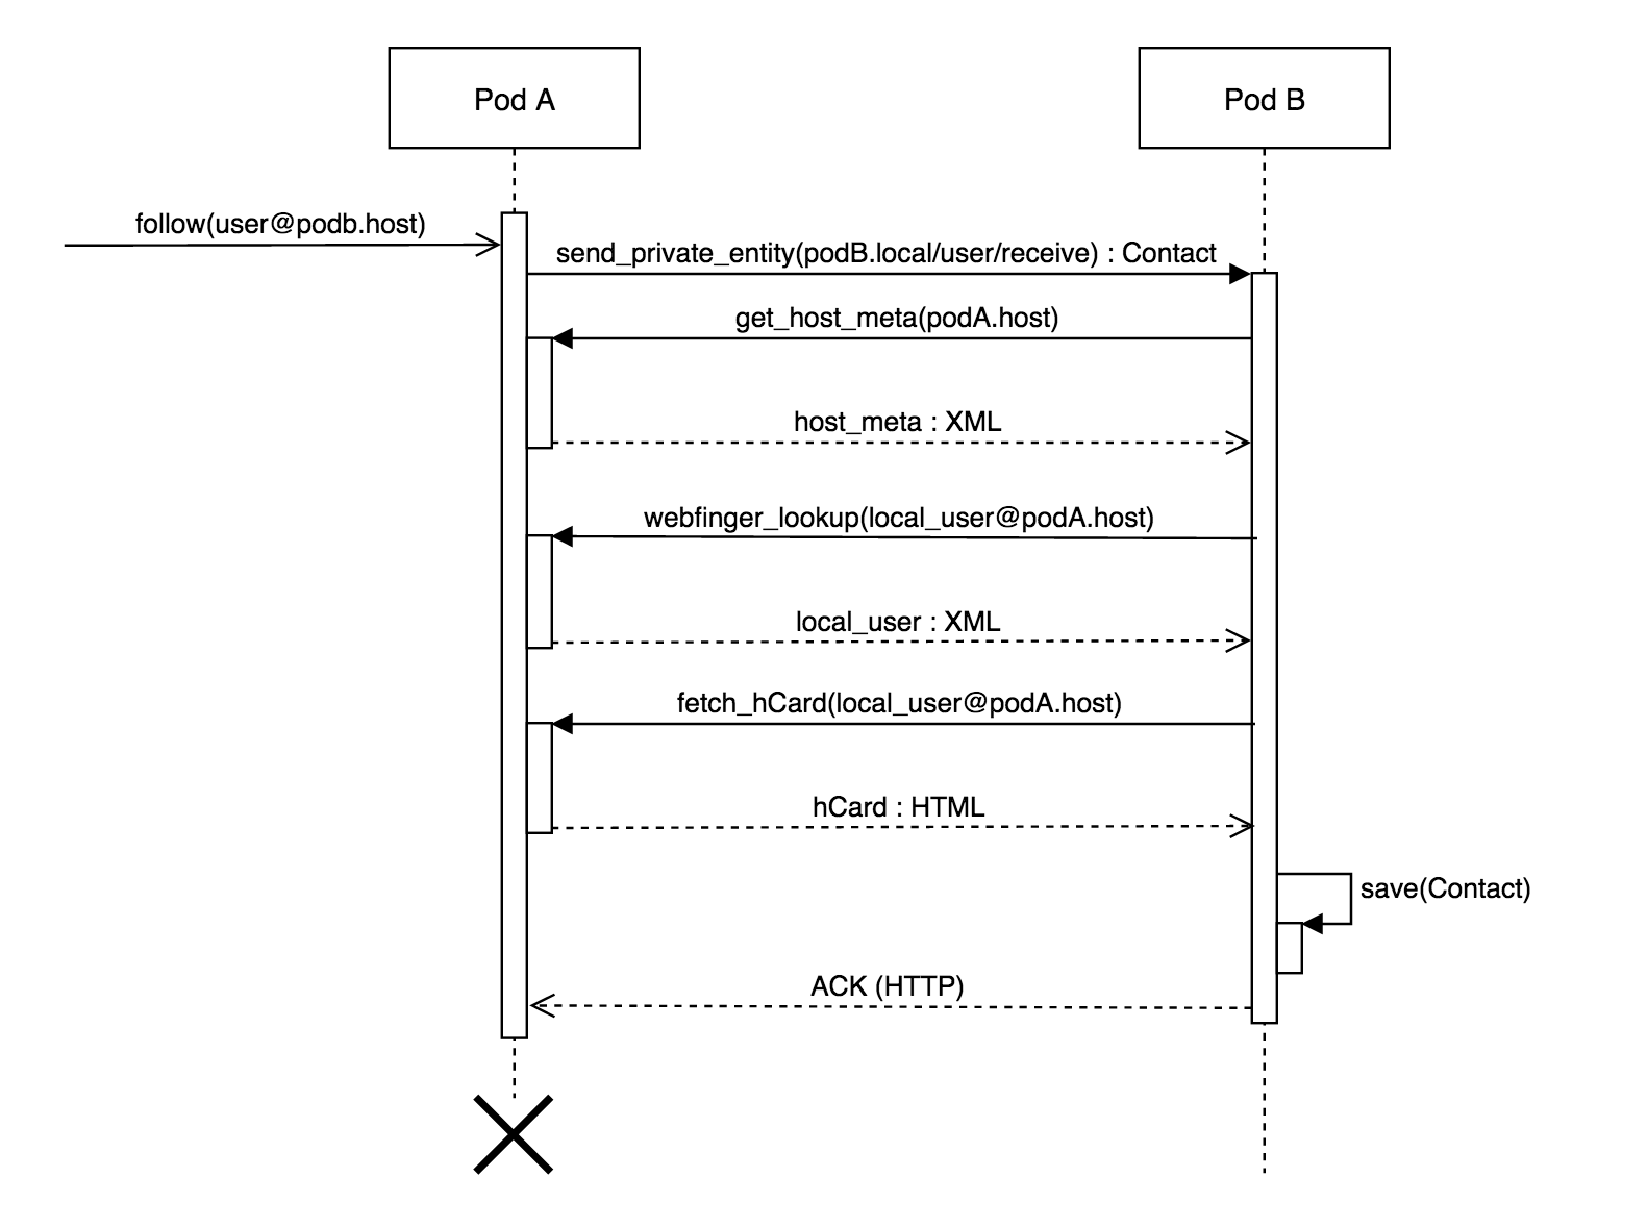
\includegraphics[keepaspectratio=true,scale=0.6]{figuras/seq_contato.eps}
	\caption{Diagrama de sequência do processo de compartilhamento de contatos}
	\label{fig:seq_contato}
\end{figure}

O envio da entidade de contato por meio do Salmon é realizado em \textit{background}
durante a execução da funcionalidade de seguir. É importante garantir que a mensagem
foi entregue, caso contrário o usuário é seguido no Noosfero mas a interação não foi
corretamente federada. A implementação executada programa outra execução da tarefa
após 10 minutos caso a mensagem não seja entregue. É necessário considerar um
parâmetro para o cancelamento da requisição, visto que a tarefa vai continuar a ser
programada infinitamente se o servidor de destino for desativado.

Mensagens privadas do Salmon devem ser criptografadas com RSA, portanto também é
necessário que cada usuário do Noosfero possua um par de chaves individual. As
chaves de um usuário são geradas apenas quando necessárias, o que evita o aumento do
esforço computacional na criação de usuários, ou em maiores dificuldades em uma
instalação que já possua vários usuários criados.

O par de chaves é gerado com a implementação em Ruby do OpenSSL, e inicialmente os
valores são armazenados serializados como texto em claro no banco de dados. Também
é importante encontrar uma alternativa para o armazenamento inadequado das chaves
privadas.

A biblioteca que implementa o protocolo providencia funções para a construção e
assinatura de mensagens Salmon, o que foi suficiente para o envio de contatos. O
Diaspora já foi capaz de reconhecer o servidor do Noosfero, criar os perfis remotos,
e exibir as notificações da interação.

% TODO: imagens

O último passo foi consumir as publicações dos usuários do Diaspora. Como pode ser
visto na Figura \ref{fig:seq_publicacao}, novos conteúdos são enviados a todos os
os servidores assinados naquela interação, no caso redes de origem de usuários que
sigam o autor. Priorizou-se a federação de conteúdos públicas, e neste caso uma
mensagem Salmon pública é enviada para o servidor Noosfero.

\begin{figure}[h]
	\centering
		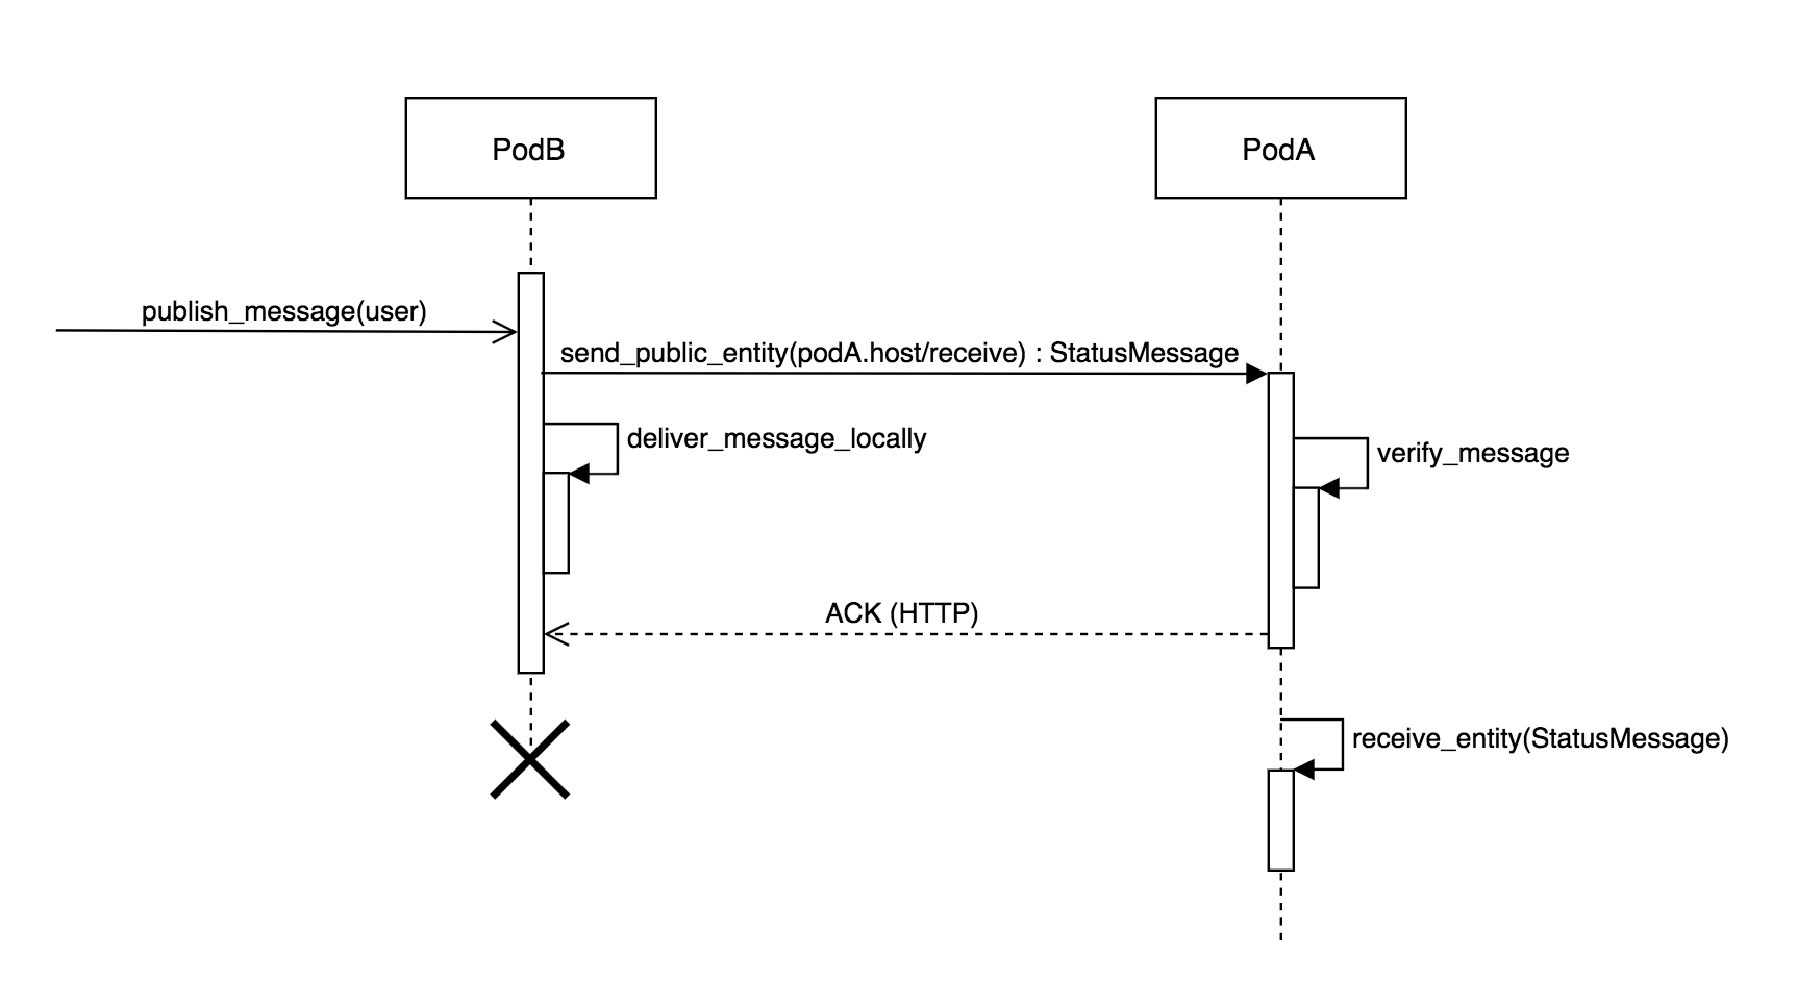
\includegraphics[keepaspectratio=true,scale=0.6]{figuras/seq_publicacao.eps}
	\caption{Diagrama de sequência do envio de publicações entre servidores}
	\label{fig:seq_publicacao}
\end{figure}

As publicações do Diaspora foram representadas no Noosfero como \textit{scraps}, que
originalmente eram publicadas apenas por perfis locais. Foi necessário evoluir as
relações da camada de domínio, permitindo que usuários externos também publicassem
novos \textit{scraps}, e adicionar um atributo GUID, um identificador universal,
obrigatórios em todas as entidades federadas através do protocolo Diaspora.

Com essas modificações, é possível criar um \textit{scrap} para o usuário externo a
partir da requisição do Diaspora. A publicação é visível apenas no perfil do usuário
externo, já que o Noosfero ainda não conta com um mecanismo de \textit{feed} ou
notificação de publicações de perfis seguidos.

Todas as modificações descritas nesta seção foram efetuadas no código \textit{core}
do Noosfero. Algumas necessidades, como por exemplo montar as rotas das ações da
federação na raiz do \textit{host}, podem dificultar a construção do código em um
\textit{plug-in}. Ainda assim, a federação poderia ser desenvolvida em um destes
componentes com modificações menores no \textit{code}, caso a comunidade julgue mais
adequado.

% TODO: Comentar sobre o código depreciado utilizado no Diaspora
% Ex.: Maginc Envelopes vs Encrypted Slaps
